\chapter{Continuous Micromagnetics}
\label{sec:cont-micromag}

In this section we give an introduction to micromagnetics including a statement of the equations to be solved.

\section{Definitions}
We use S.I. units throughout unless otherwise specified. In particular normalised quantities are no longer in S.I. units.

We define $\Hv(\xv,t)$ to be the magnetic field at position $\xv$ and time $t$ in units of $\Hu$.

We define $\Mv(\xv,t)$ to be a vector field representing the expectation value of the magnetisation per unit volume averaged over a number of unit cells.\cite{Aharoni1996}
The units of $\Mv$ are $\Mu$, the length of $\Mv(\xv,t)$ is given by the saturation magnetisation $M_s$.
At zero temperature $M_s$ is a fixed parameter of the material but in finite temperature models $M_s$ may vary.

These quantities are related to the magnetic flux density $\Bv(\xv,t)$ (in units of $\Bu$) by
\begin{equation}
  \label{eq:37}
  \Bv(\xv,t) = \mu_0 \left( \Hv(\xv,t) + \Mv(\xv,t) \right),
\end{equation}
% \cite{Gilbert2004} says that this magnetisation is different - averaged over all material rather than over a few cells...
where $\mu_0$ is the magnetic constant (or permeability of free space).

In general we will not make dependencies on $\xv$ and $t$ explicit.

\section{Energy of a Magnetic Body}
\label{sec:energy-magnetic-body}

The effects that must be considered in a micromagnetic mode are: the magnetostatic self field, the exchange energy and the magnetocrystalline anisotropy energy. Also important is the external applied field due to magnetic bodies or electrical currents outside the modelled region. Other effects which are sometimes important include temperature (thermal effects) and magnetostriction energy (due to stretching or compressing the magnet).

We begin by providing a description of each of these effects and their contribution to the total energy density, $E$. We can get the effective fields given by these energies by taking
\begin{equation}
  \Hv = \dfrac{-1}{\mu_0 V_{\magd}} \dfrac{\delta E}{\delta \Mv},
\end{equation}
where $\delta$ indicates a variational derivative and $V_{\magd}$ is the volume of the magnetic domain. ??ds citation? Is this correct?

%% Energy and field expressions below are taken from Matteo Franchin's thesis.\cite{Franchin2009}\footnote{Note that due to the variety in unit systems, definitions of magnetisation and other choices it can be difficult to compare energy/effective field equations from different authors, in particular the location of factors of $\mu_0$.}

\subsection{Exchange Energy}

In a ferromagnetic material neighbouring magnetic moments prefer to align parallel to each other due to quantum mechanical effects. This can be well approximated by a classical expression for exchange energy:\cite{Aharoni1996}
\begin{equation}
  \label{eq:39}
  \Eex =  \frac{\Exchc}{M_s^2} \int_{\magd} (\nabla M_x)^2  + (\nabla M_y)^2  + (\nabla M_z)^2 \d \magd,
\end{equation}
where $A$ is the material dependant exchange constant which depends on the crystal structure and the strength of the exchange coupling between electrons in the material.

We write the vector Laplacian as $\lap \Mv = (\lap M_x,\lap M_y, \lap M_z )$. Then the exchange effective field is given by
\begin{equation}
  \label{eq:Hex}
  \Hex = \frac{2 \Exchc}{ \mu_0 M_s} \lap \Mv.
\end{equation}

\subsection{Magnetostatic Field}
\label{sec:magnetostatic-field}

Magnetic materials generate magnetic fields, which in turn affects the magnetic material. This type of field is also known as the demagnetising field since it tends to oppose the magnetisation of the body. The magnetostatic field, $\Hms$, can be calculated in two ways: an integral based method or a potential based method. These methods are discussed in Sections~\ref{sec:magstat-field-calc-inte} and \ref{sec:magstat-field-calc-pote} respectively.

Once the self field has been calculated the energy contribution due to it is given by
\begin{equation}
  \label{eq:41}
  \Ems =  \frac{-\mu_0}{2} \int_{\magd} \Mv \cdot \Hms \d \magd,
\end{equation}
where the factor of $\frac{1}{2}$ is to avoid double counting.

The integral form of the magnetostatic field at a point $\xv \in \real^d$ due to the magnetic body $\magd$ with boundary $\boundd$ can be given in terms of magnetisation $\Mv$ by an integral over all volume and surface ``magnetic charges'' ($\nabla \cdot \Mv(\xv)$ and $\Mv(\xv) \cdot \nv(\xv)$ respectively) as
\begin{align}
  \Hms(\xv) &= \frac{1}{4 \pi} \Big[ - \int_\magd \frac{\big( \nabla' \cdot \Mv(\xv') \big)(\xv - \xv')}{\abs{ \xv -\xv'}^3} \d^3 \xv'
              + \int_\boundd \frac{ \big( \Mv(\xv') \cdot \nv(\xv') \big) (\xv - \xv')}{\abs{\xv - \xv'}^3} \d^2 \xv' \Big],
              \label{eq:Hmsint}
\end{align}
where $\nabla'$ denotes the grad operator with respect to the $\xv'$ coordinate.
For completeness we note that single magnetic charges (magnetic monopoles) have not been observed in nature.
However they are a very useful mathematical tool for calculations of magnetic fields.

% Alternatively it can be given in terms of a sum over the dipole fields of magnetic moments (\ie discretised magnetisation) as
% \begin{equation}
%   \label{eq:9}
%   \Hms(\xv) = \frac{1}{4\pi} \sum_i \frac{1}{|\xv - \xv_i|^3} \Big[ \mu_i(\xv_i) - 3(\mu_i(\xv_i) \cdot \ruv_i ) \cdot \ruv_i \Big],
% \end{equation}
% where $\ruv_i$ is the unit vector pointing from $\xv_i$ to $\xv$.


When the magnetic field is being produced only by magnets and not currents (\ie the magnetic field is irrotational) it is possible to express the field as a function of a scalar potential, $\phim$.\cite{Coey2010}
Let $\magd$ be the magnetic body, $\boundd$ it's boundary and $\nv$ the outward unit normal on the boundary.
Then we have
\begin{gather}
  \Hms = - \nabla \phim,  \label{eq:Hms} \\
  \lap \phim = \nabla \cdot \Mv \quad \xv \in \fulld, \label{eq:nnphim}
\end{gather}
With the following boundary conditions
\begin{gather}
  \phim^\inte - \phim^\exte = 0 \quad \xv \in \boundd, \label{eq:cont-phi-bound} \\
  \pd{\phim^\inte}{\nv} - \pd{\phim^\exte}{\nv} = \Mv \cdot \nv \quad \xv \in \boundd,
  \label{eq:nndphidn-bound} \\
  \phim \rightarrow 0 \text{ as } \abs{\xv} \rightarrow \infty, \label{eq:phi-inf}
\end{gather}
where $\phim^\inte$/$\phim^\exte$ are the values of $\phim$ just inside/outside the domain, $\magd$.


Similarly any external applied field gives an energy contribution of
\begin{equation}
  \label{eq:42}
  \Eapp = - \mu_0 \int_{\magd} \Mv \cdot \Happ \d \magd.
\end{equation}

\subsection{Magnetocrystalline Anisotropy}
\label{sec:magn-anis}

Many magnetic materials have a preferred direction (or directions) of magnetisation due to their crystal structure. This is known as magnetocrystalline anisotropy. The equation for the magnetocrystalline anisotropy energy depends on the crystal structure of the material.

A detailed description of the many varieties of magnetocrystalline anisotropy is beyond the scope of this report but can be found in various textbooks on magnetic materials.\cite{Coey2010}\cite{Aharoni1996} However, since the anisotropy term is always a simple function of $\Mv$ it is not important for the implementation of a numerical model which type is used. Hence we give only the most useful case: in magnetic data recording we are interested in materials with a single \emph{easy axis} either in the plane of the disk or perpendicular to it since magnetisation is most stable in these types of material. The first order approximation for the free energy contribution for a perpendicular uniaxial material is given by
\begin{equation}
  \Eca = K_u \int_\magd 1 - \left( \mv \cdot \ev \right)^2 \d \magd,
  \label{eq:36}
\end{equation}
where $\ev$ is the easy axis and $K_u$ is the (material dependant) first order anisotropy energy density coefficient.\footnote{It is possible to define many different forms for this energy. Be warned that the choice of definition changes the meaning of $K_u$!} The first order approximation is valid when the anisotropy energy density coefficients are such that $K_u = K_1 >> K_2$, which is the case in most materials.\cite{Kronmuller2003} The effective field corresponding to this case is
\begin{equation}
  \Hca = \frac{2 K_u}{\mu_0 M_s} \left( \mv \cdot \ev \right) \; \ev.
  \label{eq:Hca}
\end{equation}


\section{Core Models}
??ds before energy/fields?

The general aim of a micromagnetic model is to predict the behaviour of a magnetic body under a variety of conditions. This can either be done by finding the minimum energy of the body or by modelling the dynamics of the magnetisation.

\begin{figure}[ht!]
  \centering
  \begin{tikzpicture}[level 1/.style={sibling distance=6cm},
    level 2/.style={sibling distance=5cm}]
    \node[block] {\textbf{Micromagnetics models}}
    child {node[block] {Energy Based}}
    child {node[block] {Dynamic}
      child {node[block] {Landau--Lifshitz Equation}}
      child {node[block] {Landau--Lifshitz--Gilbert Equation}}
    };
  \end{tikzpicture}
  \caption{Possible approaches of a standard numerical micromagnetic model.}
  \label{fig:types-micromag-model}
\end{figure}


\subsection{Energy Based Micromagnetics}
\label{sec:energy-based-micr}

Energy based methods find an equilibrium state of the magnetic system by finding the minimum energy with respect to variation of $\Mv$. For example Fredkin and Koehler used a finite element energy minimisation method.\cite{Koehler1992} Energy based methods require less computational effort than dynamic methods. However they cannot give any information about the time evolution of a system.\cite{Fidler2000} This is an important problem in many areas: for example in magnetic data storage the time taken to reverse the magnetisation of a bit is of key interest.

% could include more details on how to search for minima.

\subsection{Dynamic Micromagnetics}
\label{sec:land-lifsch-gilb}

Dynamic micromagnetic methods model the time evolution of the magnetisation, for given effective field, as a differential equation. Starting with the quantum mechanical angular momentum of an electron, and converting from a single spin a continuous magnetisation gives\cite{Kronmuller2003}
\begin{equation}
  \label{eq:38}
  \dMdt = - \gymagc \Mv \times \Hv,
\end{equation}
where $\Hv$ is the total effective field
\begin{equation}
  \Hv = \Happ + \Hca + \Hex + \Hms.
  \label{eq:Heff}
\end{equation}
Equation~\eqref{eq:38} represents the procession of the magnetisation about the effective field, as shown in Figure~\ref{fig:LLG-terms}. Other effective fields can be added to equation~\eqref{eq:Heff} to model other physical effects such as finite temperature or magnetostriction.

However equation~\eqref{eq:38} implies that the precession motion is undamped, \ie no energy is lost and the magnetisation continues to precess forever. This is obviously not the case so an empirical damping term is added:
\begin{equation}
  \label{eq:LL}
  \dMdt = - \gymagc \Mv \times \Hv - \frac{\dampc \gymagc}{M_s} \Big( \Mv \times (\Mv \times \Hv) \Big),
\end{equation}
where $\dampc$ is an experimentally determined material parameter related to the strength of the damping. Equation~\eqref{eq:LL} is referred to as the Landau--Lifshitz.\cite{Landau1935} The effects of the precession and damping terms are shown in Figure~\ref{fig:LLG-terms}.

\begin{figure}[ht!]
  \centering
  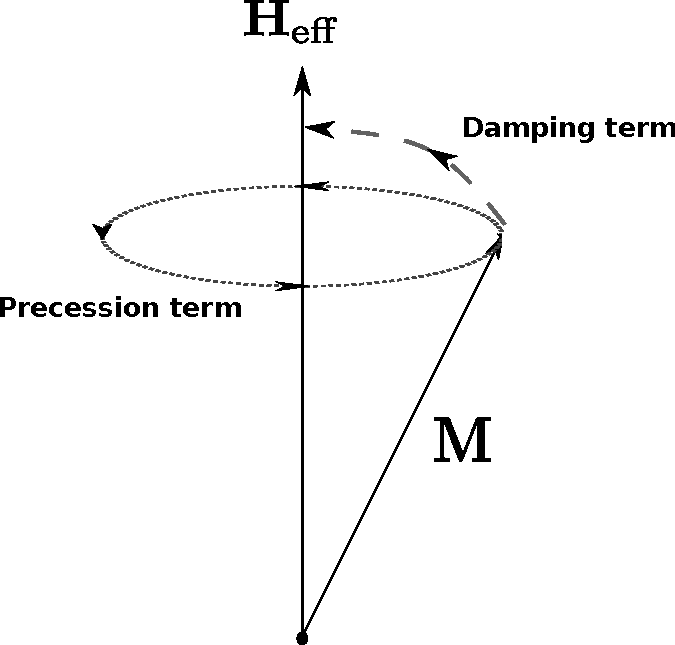
\includegraphics[width=0.6\textwidth]{./images/LLG-terms}
  \caption{The effects of the precession and damping terms in the Landau--Lifshitz and Landau--Lifshitz--Gilbert equations on the magnetisation direction, $\Mv$, of a single magnetic moment with a constant effective field
.}
  \label{fig:LLG-terms}
\end{figure}

However, there are still problems with this equation: for large damping the overall speed of the
motion increases without any increase in the precession speed. Hence the damping dominates and the switching time increases as damping is increased which is physically incorrect.\cite{Mallinson1987} There is another form of equation~\eqref{eq:LL} due to Gilbert\cite{Gilbert2004}, called the Landau--Lifshitz--Gilbert equation, which does not suffer from this problem
\begin{equation}
  \label{eq:Gilbert}
  \dMdt = - \gymagc \Mv \times \Hv + \frac{\dampc}{M_s} (\Mv \times \dMdt),
\end{equation}
where $\dampc \neq \dampc_L$. Equation~\eqref{eq:Gilbert} can be rearranged into the same form as equation~\eqref{eq:LL}, giving
\begin{equation}
  \label{eq:LLG}
  %\tag{LLG}
  \dMdt = \frac{-\gymagc}{1 + \dampc^2} \Big[ (\MxH) + \frac{\dampc}{M_s} \Big(\Mv \times (\MxH) \Big) \Big].
\end{equation}

Equations~\eqref{eq:LL}, \eqref{eq:Gilbert} and \eqref{eq:LLG} link the unknown magnetisation vector as a function of time $\Mv(t)$ with the effective field $\Hv$. To determine $\Mv$ at an arbitrary time $t \neq 0$ we need to integrate one of the above equations with respect to time. This is usually done numerically by employing a time discretisation method as discussed in Section~\ref{sec:time-discretisation}.

Note that there is no spatial dependence directly contained in equations~\eqref{eq:LL}, \eqref{eq:Gilbert} and \eqref{eq:LLG}. However the exchange effective field and magnetostatic field do contain spatial dependence, so usually the final equation to be solved after all substitutions really is a partial differential equation.

Examples of currently available micromagnetic models include the \texttt{OOMMF}\cite{oommf-website} and \texttt{nmag}\cite{Fischbacher2007} packages, which both use the dynamic method exclusively, along with \texttt{magpar}\cite{Scholz2003} and \texttt{FEMME}\cite{suessco-website} which can use either dynamic or energy based methods.


\subsubsection{Magnetisation boundary conditions}
\label{sec:magn-bound-cond}

The boundary condition on the magnetisation $\mv$ (in dimensional form) is \cite[pgs. 178, 181]{Aharoni1996}
\begin{equation}
  \Mv \times \bigb{ C \dMdn + \pd{w_s}{\Mv}} = \zerov,
\end{equation}
where $C$ is some exchange coeff ??ds and $w_s$ is the surface anisotropy.
Equivalently
\begin{equation}
    \Mv \times \dMdn = \frac{-1}{A} \Mv \times \pd{w_s}{\Mv}.
\end{equation}

For simplicity we commonly consider the case of zero surface anisotropy ($w_s \equiv 0$), in this case the boundary condition becomes
\begin{equation}
  \label{eq:llg-bc}
  \Mv \times \dMdn = \zerov.
\end{equation}
This condition can be arranged into a simpler form: we first note that for equation~\eqref{eq:llg-bc} to hold either $\Mv = \zerov$, $\dMdn = \zerov$ or $\Mv$ is parallel to $\dMdn$.
Clearly $\Mv$ is not the zero vector inside the ferromagnet.
Also we know that the magnetisation length does not change, so $\pd{\Mv}{\av} \cdot \Mv = 0$ for any direction $\av$ since the change in magnetisation projected onto the magnetisation direction is the change in magnetisation length.
Hence $\Mv$ and $\dMdn$ cannot be parallel and so
\begin{equation}
  \dMdn = \zerov.
\end{equation}

% \section{Accounting for Thermal Effects}
% \label{sec:thermal-effects}
% ??ds put in from other file when ready




% \subsection{Magnetostrictive Effects}
% \label{sec:magstric-effects}
% probably will never include this...


% \section{Limitations of Micromagnetics}
% ??ds put in from another file when ready


%%% Local Variables:
%%% mode: latex
%%% TeX-master: "./main"
%%% End:
